\documentclass[12pt,a4paper]{article}
\usepackage{amsmath,amssymb}
\usepackage{caption}
\usepackage{subcaption}
\usepackage{graphicx}
\usepackage{hyperref}
\usepackage{float}

\usepackage[margin=0.75in]{geometry}
  
\newcommand{\brac}[1] {\!\left(#1\right)}

\newcommand{\rsb}{r_{sb}}

\begin{document}
We investigate the following regularisation procedures:
\begin{equation}
\label{eq:reg_p}
\frac{1}{\brac{p^2+\Lambda^2}^{1/2}},
\end{equation}
\begin{equation}
\label{eq:reg_tanh}
\tanh\brac{\frac{p}{\Lambda}}.
\end{equation}
In both cases, the regulator \(\Lambda\) is chosen such that the value of \(\mathrm{Im}V_S\brac{r_d,\Lambda}\) reaches 99\% of its asymptotic value \(\mathrm{Im}V_S\brac{r\to\infty,\Lambda}\), where \(r_d\) is the `decorrelation length' defined via the flattening of the real part of the potential. 

Interestingly, the regulators turn out to be quite similar in both cases.
\begin{figure}[H]
	\centering
	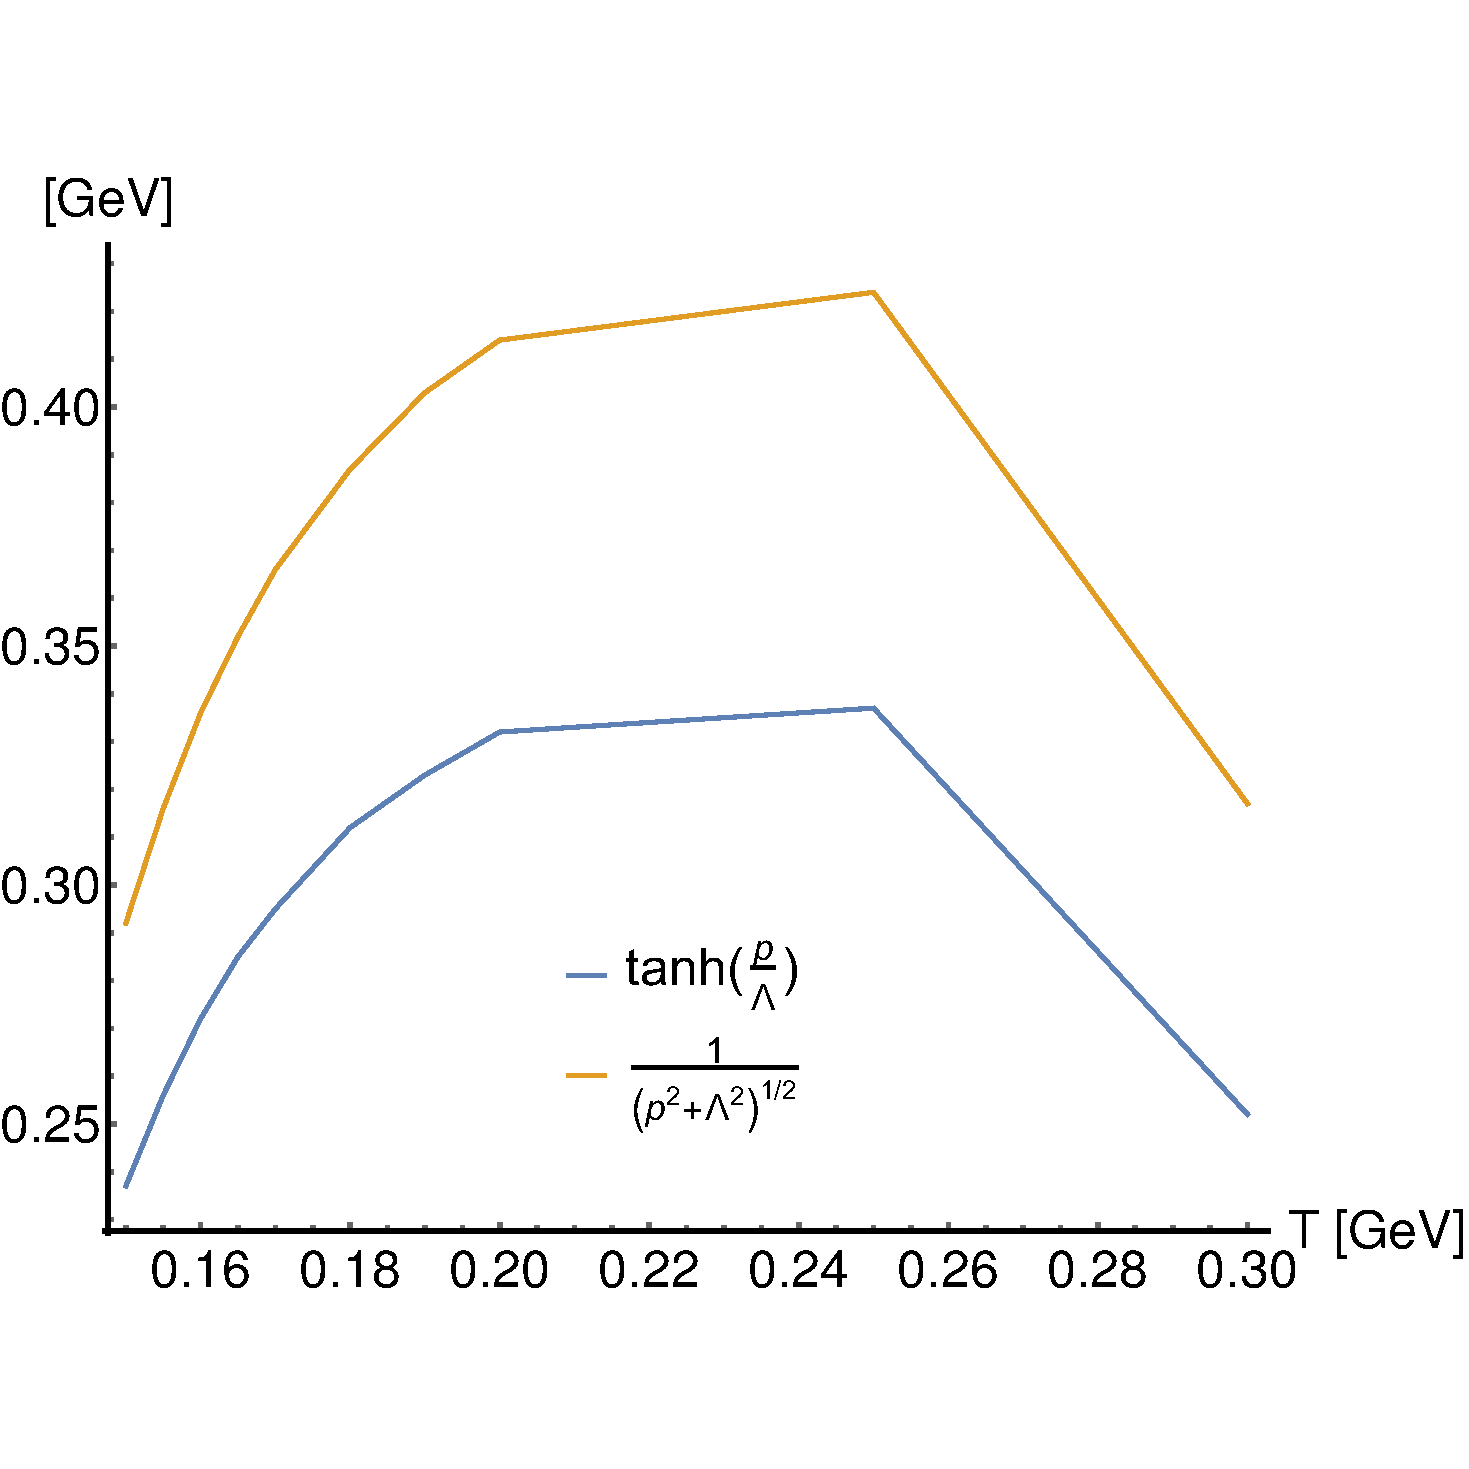
\includegraphics[width=\textwidth]{regulators} 
	\caption{Temperature dependence of the regulators in each case.}    	
	\label{fig:reg}
\end{figure}
\clearpage
Using physical values, the result from using Eq.~\eqref{eq:reg_p} is
\begin{figure}[H]
	\centering
	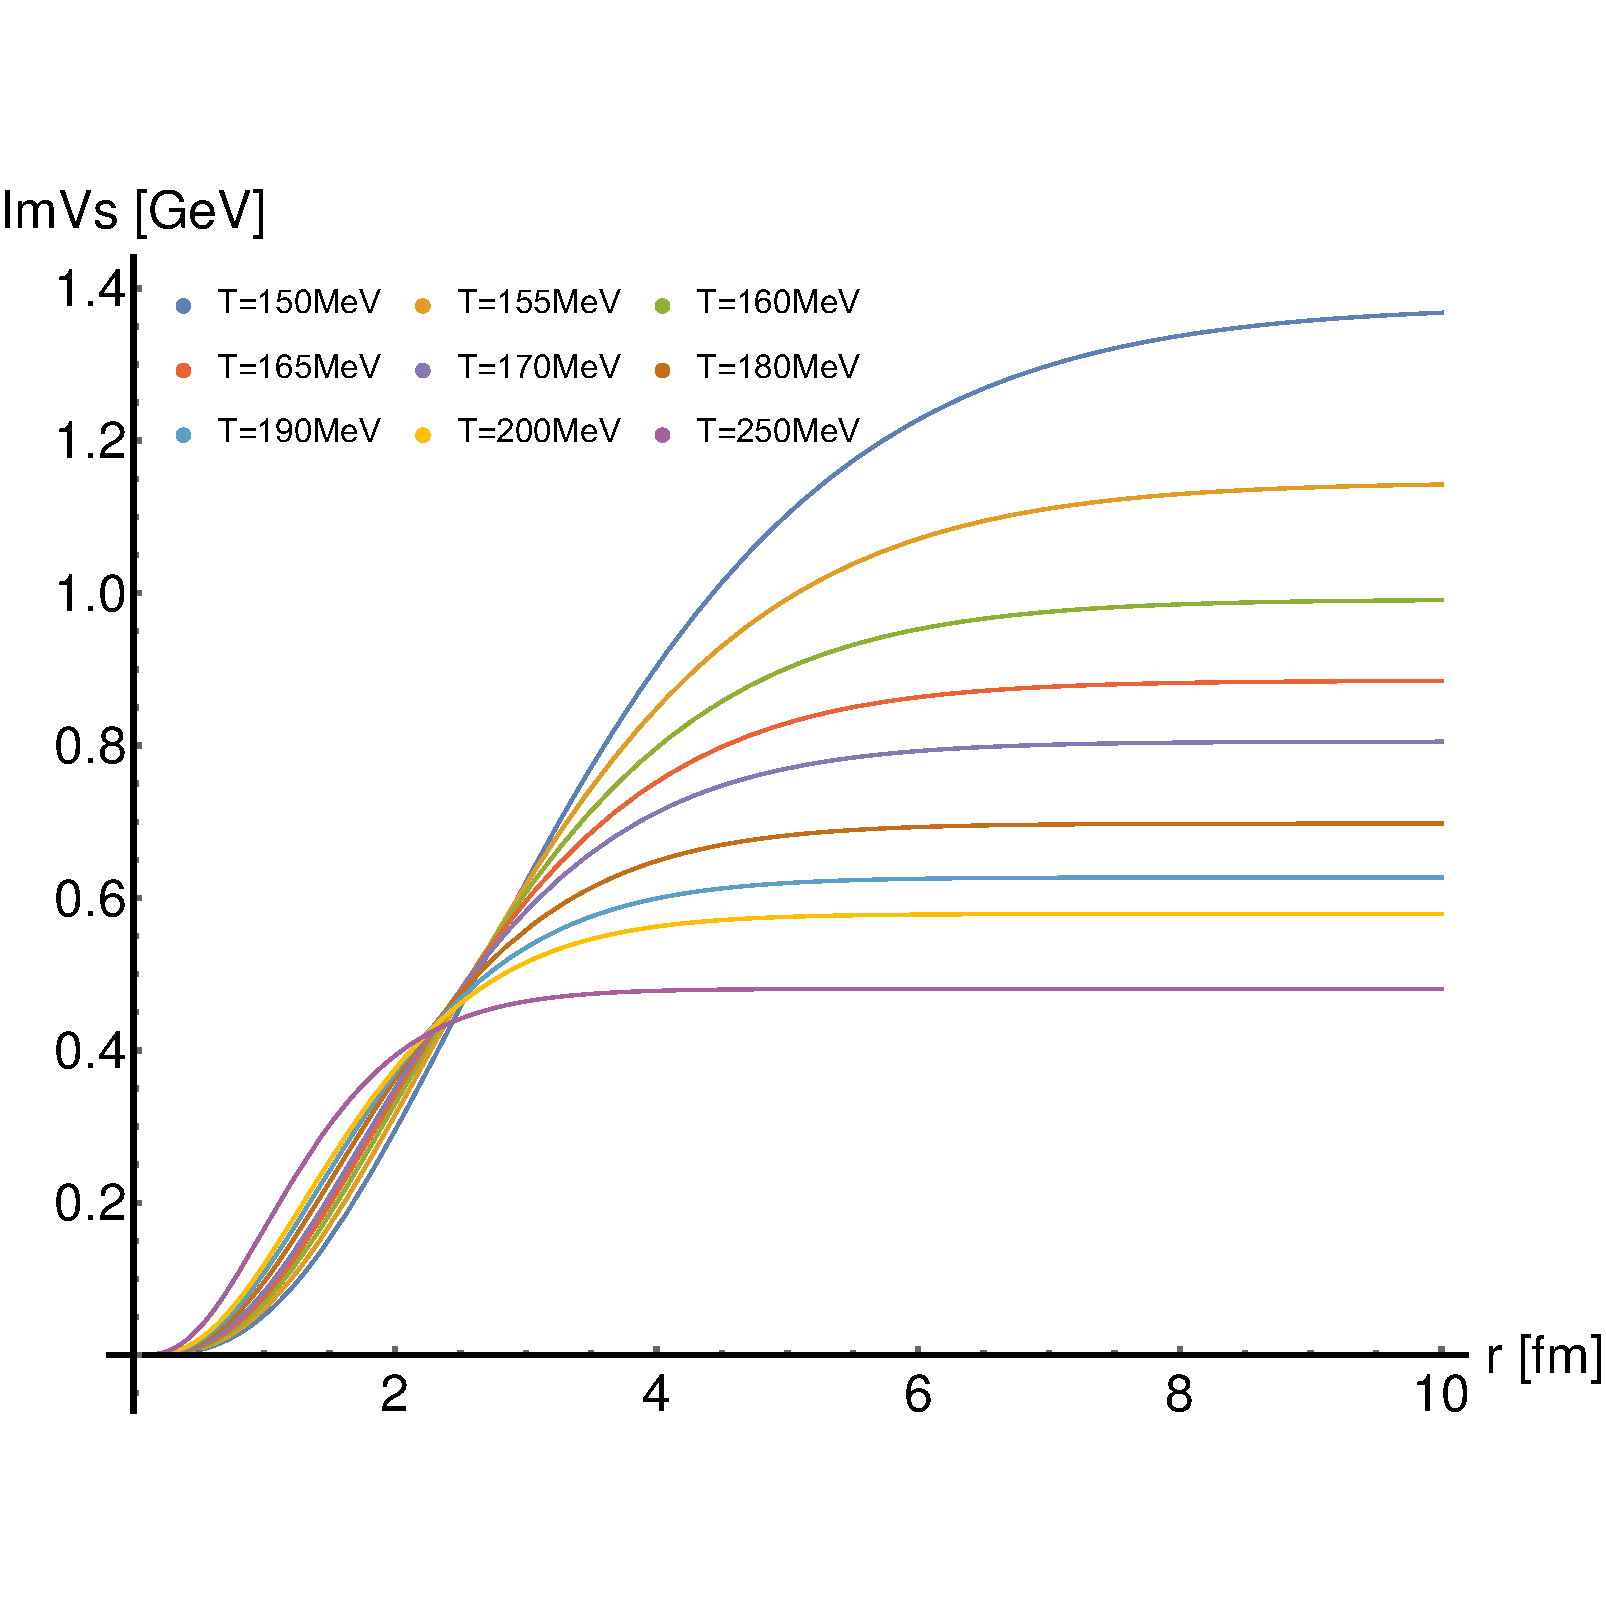
\includegraphics[width=\textwidth]{ImVs_p} 
	\caption{String imaginary part of the potential using Eq.~\eqref{eq:reg_p}.}
	\label{fig:ImVs_p}
\end{figure}
\clearpage
and from using Eq.~\eqref{eq:reg_tanh}
\begin{figure}[H]
	\centering
	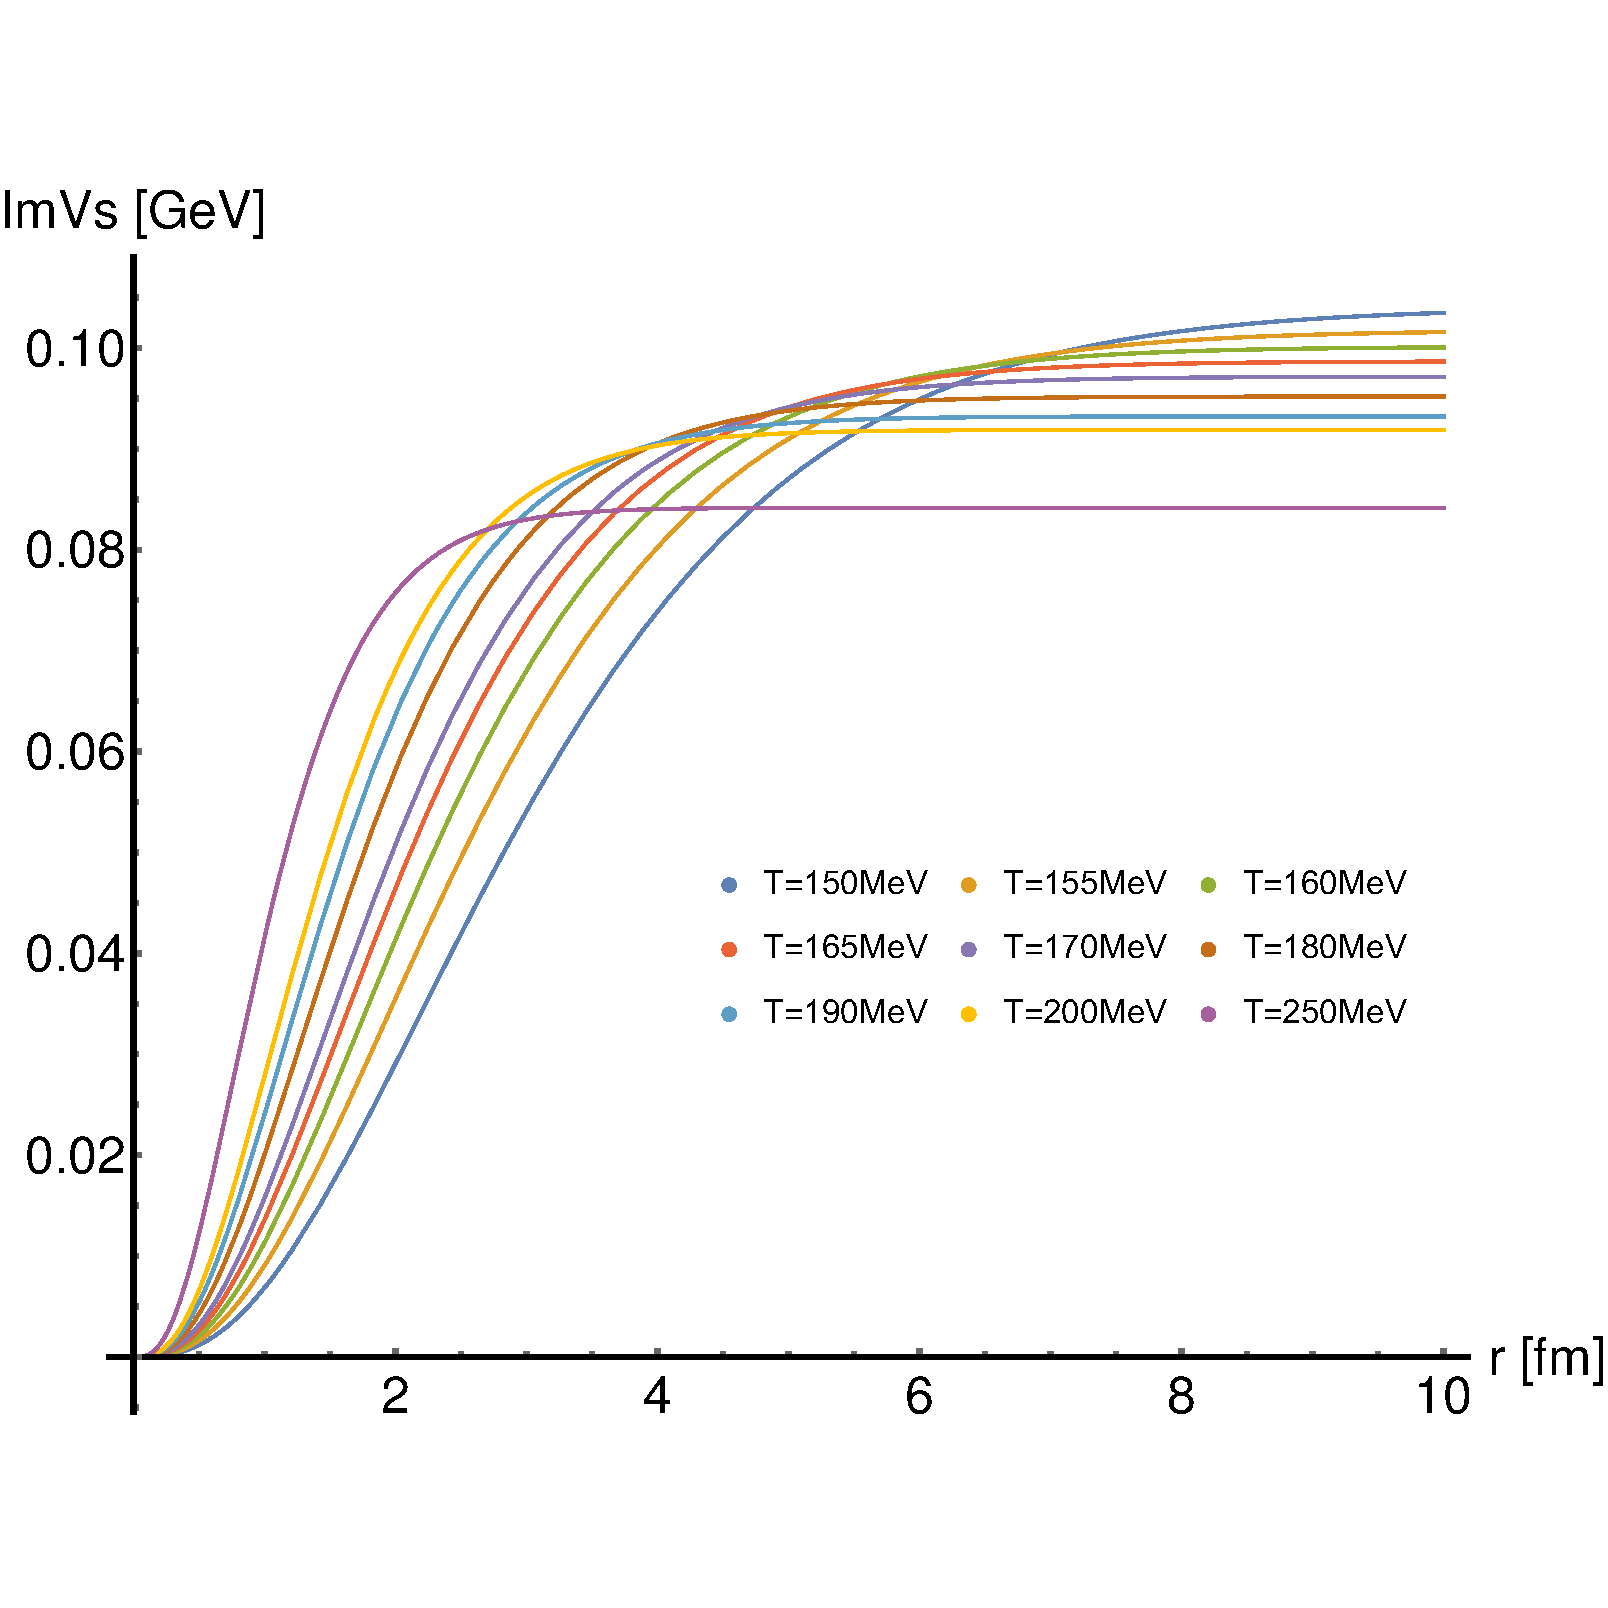
\includegraphics[width=\textwidth]{ImVs_tanh} 
	\caption{String imaginary part of the potential using Eq.~\eqref{eq:reg_tanh}.}
	\label{fig:ImVs_tanh}
\end{figure}
\clearpage
The lattice fits look as follows
\begin{figure}[H]
	\centering
	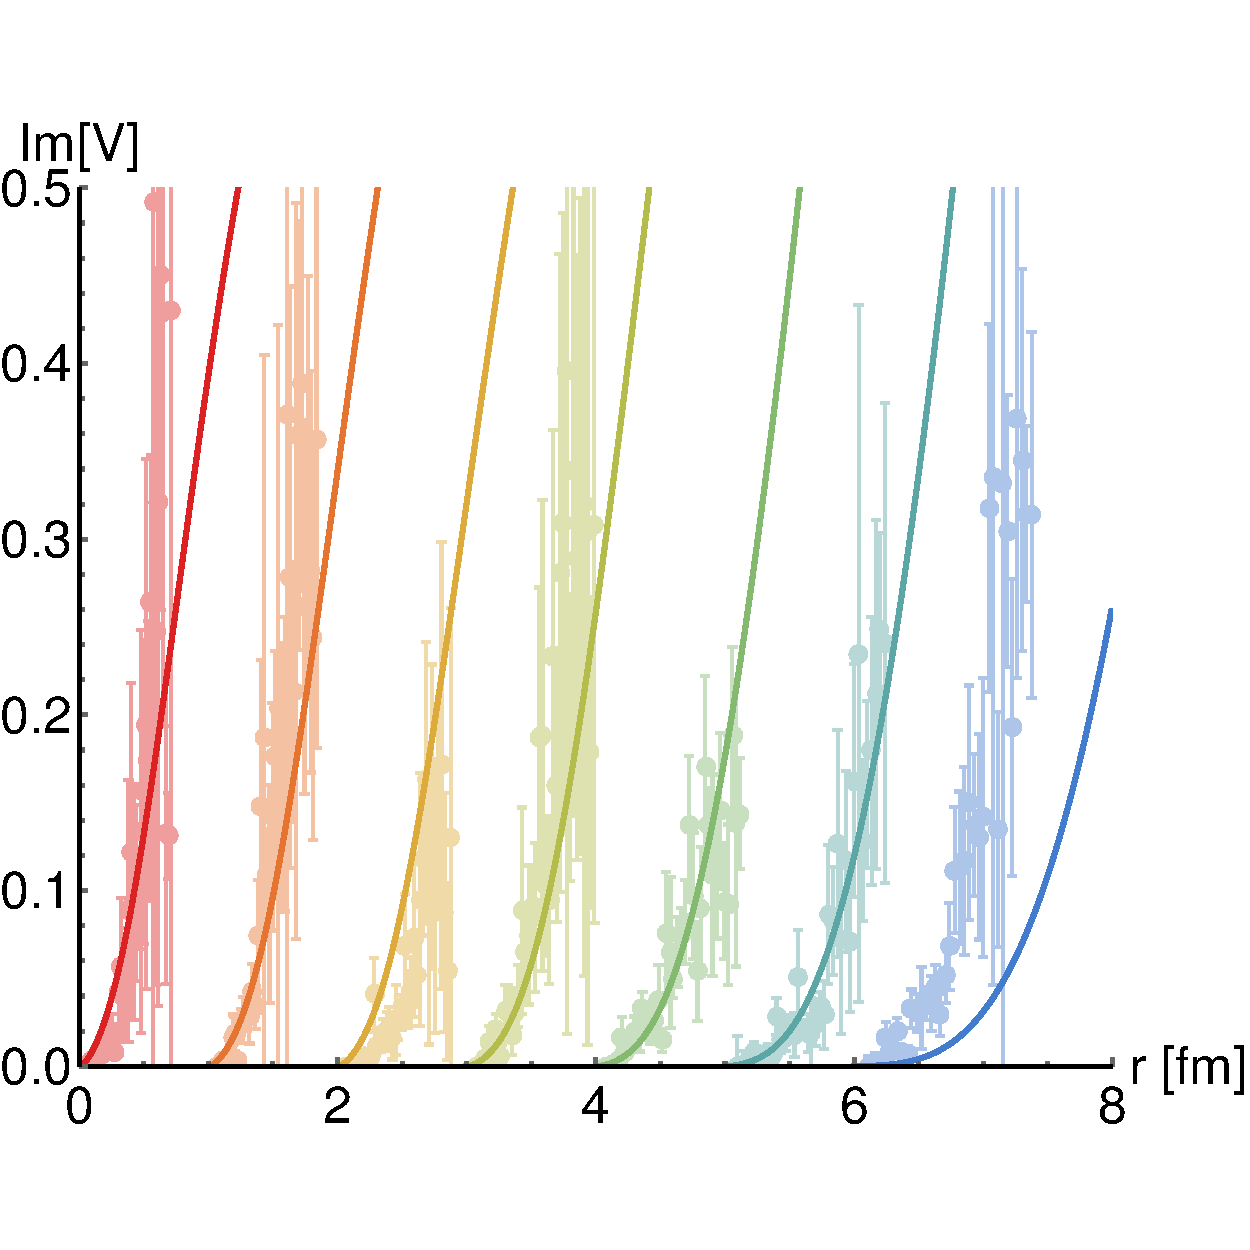
\includegraphics[width=\textwidth]{ImV_lat_p} 
	\caption{Lattice post-diction of imaginary part of the potential using Eq.~\eqref{eq:reg_p}.}
	\label{fig:ImVs_tanh}
\end{figure}
\begin{figure}[H]
	\centering
	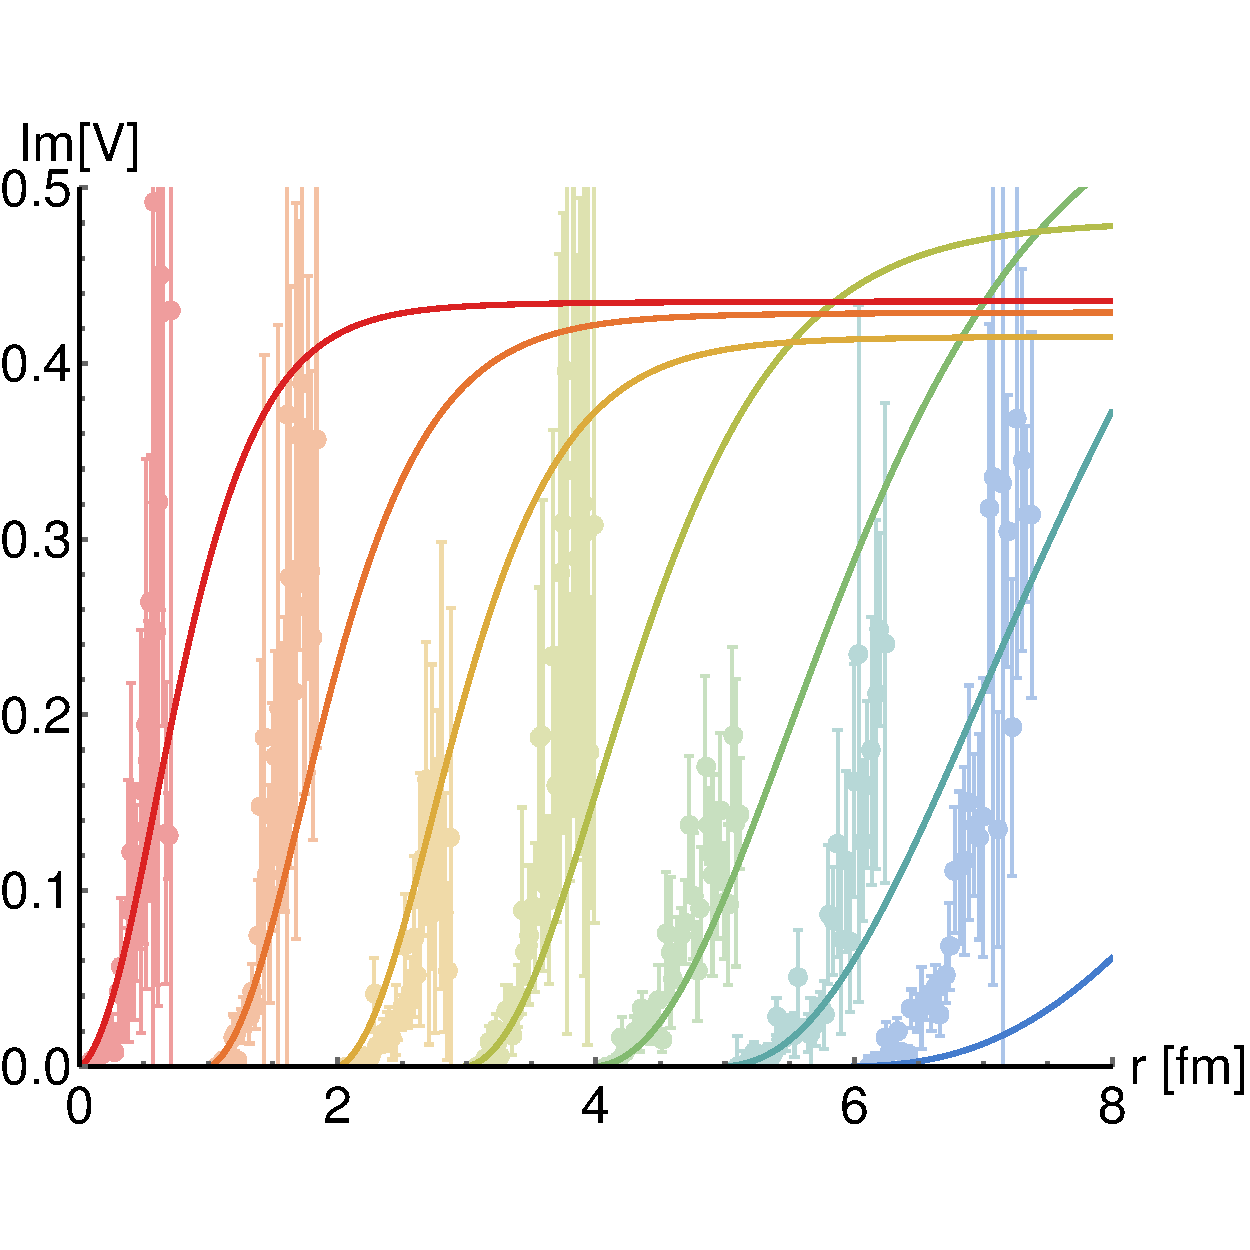
\includegraphics[width=\textwidth]{ImV_lat_tanh} 
	\caption{Lattice post-diction of imaginary part of the potential using Eq.~\eqref{eq:reg_tanh}.}
	\label{fig:ImVs_tanh}
\end{figure}
\clearpage
For lower temperatures, the hope was to implement a natural regularisation such that the string imaginary part would flatten off at the thermal string breaking radius \(r_{sb}\), defined as the separation at which the real part of the potential crosses the vacuum threshold for pair creation. However, in both cases this would require a distastefully large regulator.
\begin{figure}[H]
	\centering
	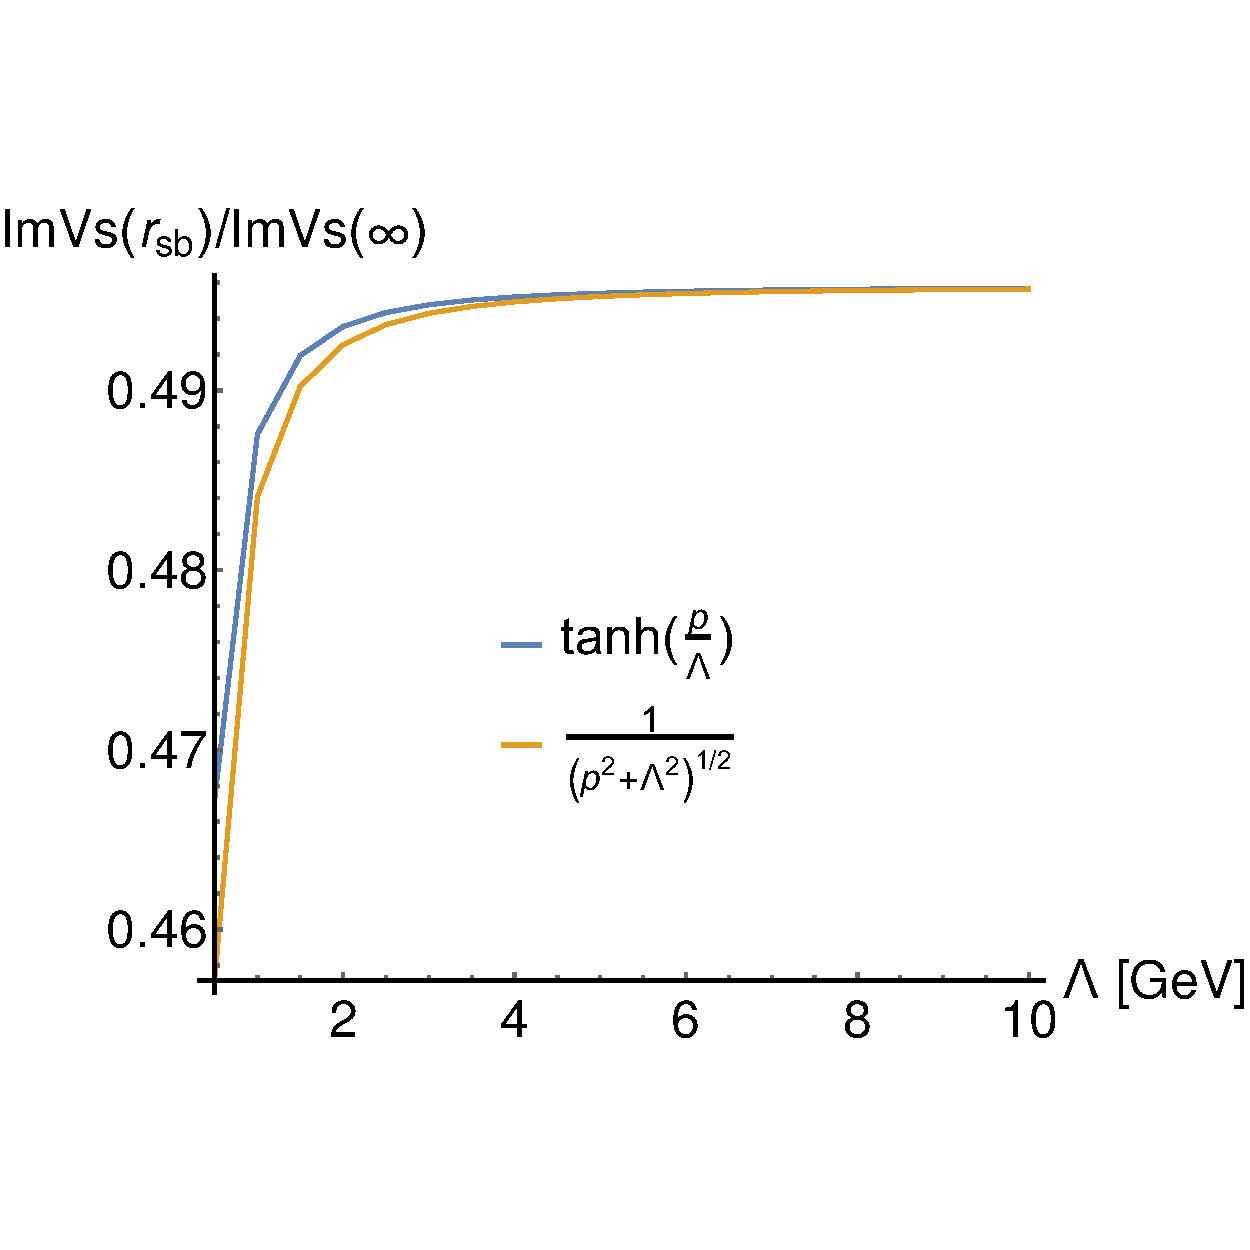
\includegraphics[width=\textwidth]{ratio} 
	\caption{Not quite there.}
	\label{fig:ratio}
\end{figure}
\end{document}